\documentclass[aspectratio=169]{beamer}

\usepackage[english]{babel}
\usepackage{newlfont}
\usepackage{color}
\usepackage{subfig}
%\usepackage{subcaption}
\usepackage{wrapfig}
\usepackage{sidecap}
\usepackage[rlft]{floatflt}
\usepackage{braket}
\usepackage{empheq}
\usepackage{xcolor}
\usepackage{amsmath}
\usepackage{amssymb}
\usepackage[mathscr]{euscript}
\usepackage[utf8x]{inputenc}
\usepackage[T1]{fontenc}
\usepackage{multirow}
\usepackage{fancyhdr}
\usepackage{tikz}
\usepackage[flushleft]{threeparttable}
\usepackage{graphicx}
\usepackage{float}
\usepackage{booktabs}
\usepackage{mdframed}
\usepackage{xcolor}
\usepackage[scale=2]{ccicons}
\usepackage{totcount}
\usetikzlibrary{positioning}

\tikzset{c-rectangle2/.style={rectangle, rounded corners, minimum width=2cm, minimum height=1cm, text centered, text width=3cm, draw=black, fill=white},
arrow/.style={thick,->,>=stealth}}


\usetheme[progressbar=frametitle]{metropolis}

%\definecolor{c1}{rgb}{0.0, 0.18, 0.39}
\definecolor{c1}{rgb}{0.36, 0.54, 0.66}
%\definecolor{c1}{rgb}{0.21, 0.25, 0.27}
%\definecolor{c2}{rgb}{0.45, 0.76, 0.98}
%\definecolor{c2}{rgb}{0.2, 0.2, 0.6}


\definecolor{c2}{rgb}{1.0, 0.49, 0.0}
%\definecolor{c1}{rgb}{0.6, 0.0, 0.0}
%\definecolor{c2}{rgb}{0.8, 0.3, 0.1}

\definecolor{c_doing}{rgb}{1.0, 0.74, 0.53}
\definecolor{c_done}{rgb}{0.98, 0.98, 0.82}
\definecolor{c_stored}{rgb}{0.68, 0.85, 0.9}

\setbeamercolor{progress bar}{bg=c1,fg=c2}
\setbeamercolor{frametitle}{bg=c1, fg=white}
\setbeamercolor{itemize item}{bg=white, fg=c2}
\setbeamertemplate{itemize item}[ball]
\setbeamercolor{background canvas}{bg=white}

\setbeamercovered{dynamic}


\title{Toy Example}
\subtitle{Permutation Closed Testing with Sum-Based Statistics}
\date{}
\author{}
\institute{}

\makeatletter
\setlength{\metropolis@progressinheadfoot@linewidth}{1pt}
\setlength{\metropolis@titleseparator@linewidth}{1pt}
\setlength{\metropolis@progressonsectionpage@linewidth}{1pt}

\setbeamertemplate{progress bar in section page}{
  \setlength{\metropolis@progressonsectionpage}{%
    \textwidth * \ratio{\thesection pt}{\totvalue{totalsection} pt}%
  }%
  \begin{tikzpicture}
    \fill[bg] (0,0) rectangle (\textwidth, \metropolis@progressonsectionpage@linewidth);
    \fill[fg] (0,0) rectangle (\metropolis@progressonsectionpage, \metropolis@progressonsectionpage@linewidth);
  \end{tikzpicture}%
}

\makeatother

\newcounter{totalsection}
\regtotcounter{totalsection}

\AtBeginDocument{%
    \pretocmd{\section}{\refstepcounter{totalsection}}{\typeout{Yes, prepending was successful}}{\typeout{No, prepending was not it was successful}}%
}%




\begin{document}
\maketitle



% ---------------------------------------------------------------------------------------------------------------------------------------%

\section{Data}
\begin{frame}{Data with 5 variables and 10 permutations}

\begin{table}[h!]
\centering
\resizebox{0.4\textwidth}{!}{
\begin{tabular}{ccccc}
\multicolumn{5}{c}{$\mathbf{G}$}\\
$(1)$ & $(2)$ & $(3)$ & $(4)$ & $(5)$\\
\cline{1-5}
28.42 & 16.68 & 9.36 & 6.12 & 9.40\\
0.10 & 0.06 & 1.37 & 0.08 & 0.56\\
0.69 & 3.07 & 4.33 & 0.83 & 0.36\\
1.07 & 30.31 & 1.11 & 8.55 & 0.26\\
0.22 & 7.45 & 2.87 & 0.48 & 1.02\\
1.83 & 0.04 & 2.85 & 0.04 & 0.02\\
17.68 & 1.82 & 6.00 & 1.52 & 1.06\\
1.77 & 26.12 & 0.29 & 0.26 & 4.07\\
2.71 & 0.37 & 8.47 & 5.83 & 4.42\\
1.14 & 0.03 & 24.06 & 8.84 & 2.41\\
\end{tabular}
}
\end{table}
We test $S=\{5\}$ with level $\alpha=0.2$
\end{frame}


% ---------------------------------------------------------------------------------------------------------------------------------------%

\section{Analysis}
\begin{frame}{Elements for the Analysis}
\begin{table}[h!]
\centering
\resizebox{\textwidth}{!}{
\begin{tabular}{ccccccccccc}
$\mathbf{d}_S$ & & \multicolumn{4}{c}{$\mathbf{D}$} & & \multicolumn{4}{c}{$\mathbf{R}$}\\
$(5)$ &  & $(4)$ & $(3)$ & $(2)$ & $(1)$ &  &  &  &  &  \\
\cline{1-1} \cline{3-6} \cline{8-11}
0.00 &  & 0.00 & 0.00 & 0.00 & 0.00 &  & 0.00 (1)& 0.00 (2)& 0.00 (3)& 0.00 (4)\\
-8.84 &  & -6.03 & -7.99 & -16.62 & -28.32 &  & -6.03 (4)& -7.99 (3)& -16.62 (2)& -28.32 (1)\\
-9.04 &  & -5.29 & -5.02 & -13.61 & -27.72 &  & -5.02 (3)& -5.29 (4)& -13.61 (2)& -27.72 (1)\\
-9.14 &  & 2.43 & -8.25 & 13.63 & -27.34 &  & 13.63 (2)& 2.43 (4)& -8.25 (3)& -27.34 (1)\\
-8.38 &  & -5.63 & -6.49 & -9.23 & -28.19 &  & -5.63 (4)& -6.49 (3)& -9.23 (2)& -28.19 (1)\\
-9.38 &  & -6.08 & -6.51 & -16.64 & -26.59 &  & -6.08 (4)& -6.51 (3)& -16.64 (2)& -26.59 (1)\\
-8.34 &  & -4.59 & -3.36 & -14.86 & -10.74 &  & -3.36 (3)& -4.59 (4)& -10.74 (1)& -14.86 (2)\\
-5.33 &  & -5.85 & -9.07 & 9.44 & -26.65 &  & 9.44 (2)& -5.85 (4)& -9.07 (3)& -26.65 (1)\\
-4.98 &  & -0.28 & -0.89 & -16.31 & -25.71 &  & -0.28 (4)& -0.89 (3)& -16.31 (2)& -25.71 (1)\\
-6.99 &  & 2.72 & 14.70 & -16.65 & -27.27 &  & 14.70 (3)& 2.72 (4)& -16.65 (2) & -27.27 (1)
\end{tabular}
}
\end{table}
\end{frame}


% ---------------------------------------------------------------------------------------------------------------------------------------%

\begin{frame}{Analysis}
$L_v$ and $U_v$ are the 8-th ordered statistics of
\begin{align*}
& \mathbf{d}_{\tilde{V}}=\mathbf{d}_S + \sum_{i=1}^v \mathbf{D}_i & \mathbf{u}_v=\mathbf{d}_S + \sum_{i=1}^v \mathbf{R}_i
\end{align*}

\vspace{3mm}
\begin{table}[h!]
\centering
\begin{tabular}{cccccc}
\toprule
$v$ & 0 & 1 & 2 & 3 & 4\\
\midrule
$U_v$ & -5.33 & 4.11 & 0.00 & -6.22 & -33.49\\
$L_v$ & -5.33 & -5.26 & -6.16 & -6.22 & -33.49\\
\midrule
rej & T & ? & ? & T & T\\
\bottomrule
\end{tabular}
\end{table}
\end{frame}


% ---------------------------------------------------------------------------------------------------------------------------------------%


\begin{frame}{Analysis}
\begin{figure}
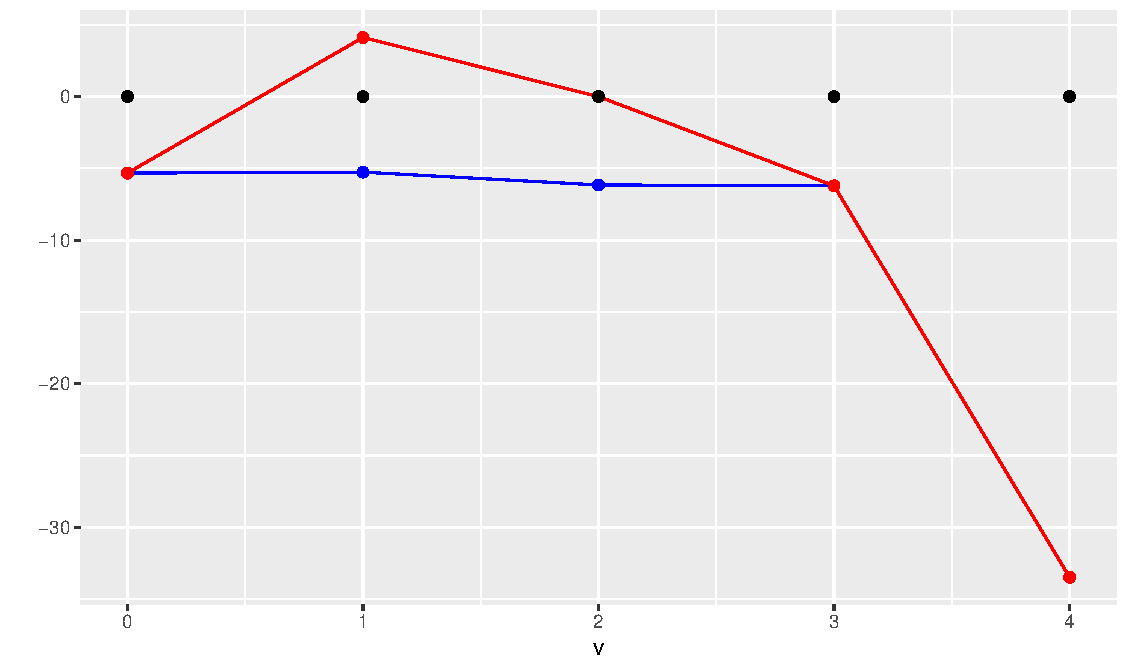
\includegraphics[scale=0.5]{plot1.pdf}
\caption{Upper (red) and lower (blue) critical values and observed values (zero, black) by additional superset size $v$.}
\end{figure}
\end{frame}


% ---------------------------------------------------------------------------------------------------------------------------------------%


\section{Branch and Bound - Lowest Statistic}

\begin{frame}{Branch and Bound - Lowest Statistic}

The total space is partitioned according to the inclusion of 4.

\vspace{3mm}
In both subspaces, $U_v$ decreases.
\begin{itemize}
\item $\mathbb{S}_{-4}$: $L_v$ may change, hence we examine both bounds
\item $\mathbb{S}_{+4}$: $L_v$ does not change, hence we examine $U_v$
\end{itemize}

\vspace{3mm}
For each node, we save:
\begin{itemize}
\item sizes $v$ to be examined (when keeping an index, $v$ decreases of 1 unit)
\item $\mathbf{R}$ and the corresponding indices
\item cumulative sums of $\mathbf{d}_S + \mathbf{d}_{\text{kept}}$ with $\mathbf{R}$ and $\mathbf{D}$
\end{itemize}
\end{frame}


% ---------------------------------------------------------------------------------------------------------------------------------------%

\begin{frame}{Removal First - Step 1}
\begin{itemize}
\item We enumerate the two subspaces: $\mathbb{S}_{+4}$ is stored, and $\mathbb{S}_{-4}$ is examined (both bounds)
\item we keep removing indices until we can close a node
\item then we start again from the node that was stored last
\end{itemize}

\vspace{3mm}
\begin{figure}[h!]
\centering
\begin{tikzpicture}[node distance = 2cm]
\node (n0) [c-rectangle2, fill=c_done] {both for $(0,\ldots,4)$\\
ind: $(1,2)$
};
\node (n1sx) [c-rectangle2, below of=n0, xshift=-4cm, fill=c_doing] {both for $(1,2)$\\
ind: $(1)$
};
\node (n1dx) [c-rectangle2, below of=n0, xshift=+4cm, fill=c_stored] {upper for $(1)$\\
stored 1st
};
\draw [arrow] (n0) -- node[anchor=east] {-(4)} (n1sx);
\draw [arrow] (n0) -- node[anchor=west] {+(4)} (n1dx);
\end{tikzpicture}
%\caption{Illustration of State of the Art}
%\label{fig:Illustration of State of the Art}
\end{figure}
\end{frame}


% ---------------------------------------------------------------------------------------------------------------------------------------%




\begin{frame}{Removal First - Step 2}
\begin{figure}[h!]
\centering
\resizebox{\textwidth}{!}{
\begin{tikzpicture}[node distance = 2cm]
\node (n0) [c-rectangle2, fill=c_done] {
both for $(0,\ldots,4)$\\
ind: $(1,2)$
};
\node (n1sx) [c-rectangle2, below of=n0, xshift=-4cm, fill=c_done] {
both for $(1,2)$\\
ind: $(1)$
};
\node (n1dx) [c-rectangle2, below of=n0, xshift=+4cm, fill=c_stored] {
upper for $(1)$\\
stored 1st
};
\node (n2sx) [c-rectangle2, below of=n1sx, xshift=-3cm, fill=c_doing] {
both for $(1)$\\
non-rejection
};
\node (n2dx) [c-rectangle2, below of=n1sx, xshift=+3cm, fill=c_done] {
not stored
};
\draw [arrow] (n0) -- node[anchor=east] {-(4)} (n1sx);
\draw [arrow] (n0) -- node[anchor=west] {+(4)} (n1dx);
\draw [arrow] (n1sx) -- node[anchor=east] {-(3)} (n2sx);
\draw [arrow] (n1sx) -- node[anchor=west] {+(3)} (n2dx);
\end{tikzpicture}
}
%\caption{Illustration of State of the Art}
%\label{fig:Illustration of State of the Art}
\end{figure}
\end{frame}




% ---------------------------------------------------------------------------------------------------------------------------------------%


\begin{frame}{Keeping First - Step 1}
We start by examining $U_v$ in $\mathbb{S}_{+4}$ (hence we cannot find any non-rejection).

\vspace{3mm}
\begin{figure}[h!]
\centering
\begin{tikzpicture}[node distance = 2cm]
\node (n0) [c-rectangle2, fill=c_done] {
both for $(0,\ldots,4)$
ind: $(1,2)$
};
\node (n1) [c-rectangle2, below of=n0, xshift=4.4cm, fill=c_doing] {
upper for $(1)$\\
ind: $(1)$
};
\node (n4) [c-rectangle2, below of=n0, xshift=-4.4cm, fill=c_stored] {
both for $(1,2)$\\
stored 1st
};
\draw [arrow] (n0) -- node[anchor=west] {+(4)} (n1);
\draw [arrow] (n0) -- node[anchor=east] {-(4)} (n4);
\end{tikzpicture}
\end{figure}
\end{frame}


% ---------------------------------------------------------------------------------------------------------------------------------------%


\begin{frame}{Keeping First - Step 2}
\begin{figure}[h!]
\centering
\resizebox{\textwidth}{!}{
\begin{tikzpicture}[node distance = 2cm]
\node (n0) [c-rectangle2, fill=c_done] {
both for $(0,\ldots,4)$
ind: $(1,2)$
};
\node (n1) [c-rectangle2, below of=n0, xshift=4.4cm, fill=c_done] {
upper for $(1)$\\
ind: $(1)$
};
\node (n2) [c-rectangle2, below of=n1, xshift=2.2cm, fill=c_done] {
not examined
};
\node (n3) [c-rectangle2, below of=n1, xshift=-2.2cm, fill=c_doing] {
both for $(1)$\\
rejection
};
\node (n4) [c-rectangle2, below of=n0, xshift=-4.4cm, fill=c_stored] {
both for $(1,2)$\\
stored 1st
};
\draw [arrow] (n0) -- node[anchor=west] {+(4)} (n1);
\draw [arrow] (n1) -- node[anchor=west] {+(3)} (n2);
\draw [arrow] (n1) -- node[anchor=east] {-(3)} (n3);
\draw [arrow] (n0) -- node[anchor=east] {-(4)} (n4);
\end{tikzpicture}
}
\end{figure}
\end{frame}


% ---------------------------------------------------------------------------------------------------------------------------------------%


\begin{frame}{Keeping First - Step 3}
\begin{figure}[h!]
\centering
\resizebox{\textwidth}{!}{
\begin{tikzpicture}[node distance = 2cm]
\node (n0) [c-rectangle2, fill=c_done] {
both for $(0,\ldots,4)$
ind: $(1,2)$
};
\node (n1) [c-rectangle2, below of=n0, xshift=4.4cm, fill=c_done] {
upper for $(1)$\\
ind: $(1)$
};
\node (n2) [c-rectangle2, below of=n1, xshift=2.2cm, fill=c_done] {
not examined
};
\node (n3) [c-rectangle2, below of=n1, xshift=-2.2cm, fill=c_done] {
both for $(1)$\\
rejection
};
\node (n4) [c-rectangle2, below of=n0, xshift=-4.4cm, fill=c_doing] {
both for $(1,2)$\\
ind: $(1)$
};
\draw [arrow] (n0) -- node[anchor=west] {+(4)} (n1);
\draw [arrow] (n1) -- node[anchor=west] {+(3)} (n2);
\draw [arrow] (n1) -- node[anchor=east] {-(3)} (n3);
\draw [arrow] (n0) -- node[anchor=east] {-(4)} (n4);
\end{tikzpicture}
}
\end{figure}
\end{frame}



% ---------------------------------------------------------------------------------------------------------------------------------------%


\begin{frame}{Keeping First - Step 4}
\begin{figure}[h!]
\centering
\resizebox{\textwidth}{!}{
\begin{tikzpicture}[node distance = 2cm]
\node (n0) [c-rectangle2, fill=c_done] {
both for $(0,\ldots,4)$
ind: $(1,2)$
};
\node (n1) [c-rectangle2, below of=n0, xshift=4.4cm, fill=c_done] {
upper for $(1)$\\
ind: $(1)$
};
\node (n2) [c-rectangle2, below of=n1, xshift=2.2cm, fill=c_done] {
not examined
};
\node (n3) [c-rectangle2, below of=n1, xshift=-2.2cm, fill=c_done] {
both for $(1)$\\
rejection
};
\node (n4) [c-rectangle2, below of=n0, xshift=-4.4cm, fill=c_done] {
both for $(1,2)$\\
indecisive: $(1)$
};
\node (n5) [c-rectangle2, below of=n4, xshift=2.2cm, fill=c_done] {
not examined
};
\node (n6) [c-rectangle2, below of=n4, xshift=-2.2cm, fill=c_doing] {
both for $(1)$\\
non-rejection
};
\draw [arrow] (n0) -- node[anchor=west] {+(4)} (n1);
\draw [arrow] (n1) -- node[anchor=west] {+(3)} (n2);
\draw [arrow] (n1) -- node[anchor=east] {-(3)} (n3);
\draw [arrow] (n0) -- node[anchor=east] {-(4)} (n4);
\draw [arrow] (n4) -- node[anchor=west] {+(3)} (n5);
\draw [arrow] (n4) -- node[anchor=east] {-(3)} (n6);
\end{tikzpicture}
}
\end{figure}
\end{frame}





% ---------------------------------------------------------------------------------------------------------------------------------------%


\section{Branch and Bound - Highest Statistic}

\begin{frame}{Branch and Bound - Highest Statistic}

The total space may also be partitioned according to the inclusion of 1.

\vspace{3mm}
As in the previous case, $U_v$ decreases in both subspaces.
\begin{itemize}
\item $\mathbb{S}_{-1}$: $L_v$ does not change, hence we examine $U_v$
\item $\mathbb{S}_{+1}$: $L_v$ may change, hence we examine both bounds
\end{itemize}

\vspace{3mm}
In this case, it takes 3 steps in both cases.
\end{frame}


% ---------------------------------------------------------------------------------------------------------------------------------------%


\section{Simulations}
\begin{frame}{Simulations ($\approx 5000$)}
$F$: $f$ variables, where a percentage $f_{*}$ is significative.\\
$S$: contains a percentage $s_{\text{size}}$ of all variables, where a percentage $s_{*}$ is significative.\\

\vspace{5mm}
\begin{itemize}
\item $f,\,B\in\{10,50,100\}$
\item $s_{\text{size}}\in\{1, 10, 20, 50, 80, 100\}$ (\%)
\item $f_{*},\,s_{*}\in\{0, 1, 10, 20, 50, 80, 100\}$ (\%)
\item $\alpha\in\{0.05,0.20\}$
\item maximum number of iterations: $10^4$
\end{itemize}
\end{frame}


% ---------------------------------------------------------------------------------------------------------------------------------------%




\begin{frame}{Simulations with $s_{*}=0,1,10,20$}
\begin{table}[h!]
\centering
\resizebox{0.8\textwidth}{!}{
\begin{tabular}{ccccccccccc}
\toprule
$s_{*}$ & $f_{*}$ & $s_{\text{size}}$ & $f$ & $B$ & $\alpha$ & non rej & RL & KL & RH & KH\\
\midrule
1 & 1 & 10 & 100 & 50 & 0.05 & T & - & \textbf{681} & 958 & - \\
1 & 1 & 10 & 100 & 100 & 0.05 & - & - & - & - & - \\
1 & 1 & 20 & 100 & 100 & 0.05 & F & - & - & \textbf{332} & \textbf{332} \\
1 & 1 & 50 & 50 & 100 & 0.20 & F & 335 & 335 & \textbf{14} & \textbf{14} \\
10 & 20 & 80 & 50 & 50 & 0.05 & T & \textbf{4} & 6 & 5 & 6 \\
20 & 20 & 20 & 50 & 10 & 0.20 & T & 545 & 18 & \textbf{9} & 93 \\
20 & 10 & 50 & 50 & 50 & 0.05 & F & 16 & 16 & \textbf{6} & \textbf{6} \\
20 & 10 & 50 & 50 & 100 & 0.05 & F & \textbf{2} & \textbf{2} & 4 & 4 \\
\bottomrule
\end{tabular}
}
\end{table}
\end{frame}

% ---------------------------------------------------------------------------------------------------------------------------------------%




\begin{frame}{Simulations with $s_{*}=50,80$}
\begin{table}[h!]
\centering
\resizebox{0.8\textwidth}{!}{
\begin{tabular}{ccccccccccc}
\toprule
$s_{*}$ & $f_{*}$ & $s_{\text{size}}$ & $f$ & $B$ & $\alpha$ & non rej & RL & KL & RH & KH\\
\midrule
50 & 10 & 20 & 50 & 100 & 0.05 & T & - & 1970 & \textbf{154} & 856 \\
50 & 10 & 20 & 100 & 50 & 0.20 & - & - & - & - & - \\
50 & 10 & 20 & 100 & 100 & 0.20 & F & - & - & \textbf{2092} & \textbf{2092} \\
50 & 50 & 20 & 10 & 50 & 0.20 & F & 15 & 15 & \textbf{8} & \textbf{8} \\
50 & 50 & 20 & 10 & 100 & 0.20 & F & 6 & 6 & \textbf{4} & \textbf{4} \\
50 & 50 & 50 & 50 & 100 & 0.20 & F & 1702 & 1702 & \textbf{38} & \textbf{38} \\
80 & 10 & 10 & 50 & 10 & 0.20 & T & - & \textbf{91} & 309 & 316 \\
80 & 20 & 20 & 50 & 50 & 0.20 & F & 3162 & 3162 & \textbf{102} & \textbf{102} \\
80 & 20 & 20 & 50 & 100 & 0.20 & F & 218 & 218 & \textbf{20} & \textbf{20} \\
80 & 20 & 20 & 100 & 10 & 0.20 & F & - & - & \textbf{86} & \textbf{86} \\
80 & 20 & 20 & 100 & 50 & 0.20 & F & - & - & \textbf{410} & \textbf{410} \\
80 & 20 & 20 & 100 & 100 & 0.20 & F & - & - & \textbf{1320} & \textbf{1320} \\
\bottomrule
\end{tabular}
}
\end{table}
\end{frame}




\begin{frame}{Simulations with $s_{*}=100$}
\begin{table}[h!]
\centering
\resizebox{0.8\textwidth}{!}{
\begin{tabular}{ccccccccccc}
\toprule
$s_{*}$ & $f_{*}$ & $s_{\text{size}}$ & $f$ & $B$ & $\alpha$ & non rej & RL & KL & RH & KH\\
\midrule
100 & 1 & 1 & 100 & 10 & 0.20 & T & - & \textbf{111} & 880 & - \\
100 & 1 & 1 & 100 & 50 & 0.20 & F & - & - & \textbf{54} & \textbf{54} \\
100 & 1 & 1 & 100 & 100 & 0.20 & F & - & - & \textbf{9144} & \textbf{9144} \\
100 & 10 & 10 & 50 & 10 & 0.20 & T & - & \textbf{91} & 236 & 972 \\
100 & 10 & 10 & 100 & 50 & 0.20 & T & - & \textbf{345} & - & - \\
100 & 10 & 10 & 100 & 100 & 0.20 & - & - & - & - & - \\
100 & 20 & 20 & 50 & 50 & 0.05 & T & 5413 & \textbf{35} & 38 & 57 \\
100 & 20 & 20 & 100 & 100 & 0.05 & F & 134 & 134 & \textbf{12} & \textbf{12} \\
100 & 50 & 50 & 10 & 50 & 0.20 & F & \textbf{4} & \textbf{4} & \textbf{4} &  \textbf{4} \\
100 & 80 & 50 & 100 & 10 & 0.20 & F & 890 & 890 & \textbf{64} & \textbf{64} \\
100 & 100 & 50 & 50 & 100 & 0.05 & T & 625 & 18 & \textbf{14} & 94 \\
100 & 100 & 50 & 100 & 10 & 0.20 & F & - & - & \textbf{92} & \textbf{92} \\
100 & 100 & 50 & 100 & 100 & 0.20 & - & - & - & - & - \\
\bottomrule
\end{tabular}
}
\end{table}
\end{frame}




\begin{frame}{Simulation Results}
When $S$ is rejected, RL=KL and RH=KH.\\
RH required the smallest number of iterations.

\vspace{3mm}
\begin{table}[h!]
\centering
\begin{tabular}{ccccc}
\toprule
 & RL & KL & \textbf{RH} & KH\\
\midrule
$d$ & 45.5 & 63.6 & \textbf{84.8} & 78.8 \\ 
$p$ & 9.1 & 24.2 & \textbf{63.6} & 54.5 \\
$M$ & 5851 & 3935 & \textbf{2012} & 2612 \\
\bottomrule
\end{tabular}
\end{table}

\vspace{3mm}
\begin{itemize}
\item $d=$ percentage of simulations where the BAB leads to a decisive outcome
\item $p=$ percentage of simulations where the setting was optimal
\item $M=$ mean of iterations (when the number exceeds the maximum, it is approximated to the maximum)
\end{itemize}
\end{frame}





\begin{frame}{Analysis Time in R}
Mean analysis time (in milliseconds) when removing the highest statistic:
\begin{table}[h!]
\centering
\resizebox{\textwidth}{!}{
\begin{tabular}{ccccccccc}
\toprule
 & \multicolumn{2}{c}{$f=10$} &  & \multicolumn{2}{c}{$f=50$} &  & \multicolumn{2}{c}{$f=100$}\\
\cline{2-3} \cline{5-6}  \cline{8-9}
 & $\alpha=0.05$ & $\alpha=0.20$ &  & $\alpha=0.05$ & $\alpha=0.20$ &  & $\alpha=0.05$ & $\alpha=0.20$ \\
\midrule
$B=10$ & 1.2 & 0.9 &  & 1.1 & 1.4 &  & 0.6 &  16.0\\
$B=50$ & 1.8 & 1.6 &  & 1.9 & 3.3 &  & 12.1 &  109.7\\
$B=100$ & 1.9 & 1.3 &  & 3.3 & 3.4 &  & 215.9 & 1129.2 \\
\midrule
mean & 1.6 & 1.3 &  & 2.1 & 2.7 &  & 76.2 & 418.3\\
\bottomrule
\end{tabular}
}
\end{table}
\end{frame}

\end{document}


%\begin{figure}
    %\centering
    %\includegraphics[scale=0.45]{estimate.pdf}
    %\label{fig:my_label}
%\end{figure}






